\documentclass{article}
\usepackage{graphicx} % Required for inserting images
\usepackage[margin=1in]{geometry}
\usepackage{bm, amsfonts, amsmath, tikz, pgfplots, amssymb}
\pgfplotsset{compat=newest, width=10cm}


\allowdisplaybreaks
\usetikzlibrary{external}
\tikzexternalize[prefix=TikzPictures]

%\usetikzlibrary{polar}

\title{32BH Notes}
\author{Brendan Connelly}
\date{January to March 2024}

\newcommand{\R}{\mathbb{R}}
\newcommand{\C}{\mathbb{C}}
\newcommand{\Z}{\mathbb{Z}}
\newcommand{\Q}{\mathbb{Q}}
\newcommand{\F}{\mathbb{F}}

\newenvironment{definition}[1]{
    \par\noindent\textbf{#1}\par\noindent
}{
    \par \vspace{0.5cm}
}

\begin{document}

\maketitle

\section*{Upper and Lower Darboux Sums $\rightarrow$ Integral}

\begin{definition}{Bounded Subset}
    A subset \( D \subset \R^n \) is bounded if there exists some \( r > 0 \) such that \( D \subset B_r(\bm{0}) \).
\end{definition}


\begin{definition}{Bounded Function}
    A function \( f : A \subset \R^n \to \R \) is bounded if its image \(\{f(\bm{x}) \mid \bm{x} \in A\}\)
    is a bounded subset of \(\R\).
\end{definition}


\begin{definition}{Boundary Point}
    A point \( \bm{x} \in \R^n \) is a boundary point of \( D \subset \R^n \) if: for all \( \varepsilon > 0 \),
    \begin{enumerate}
        \item \( B_{\varepsilon}(\bm{x}) \cap D \) is non-empty, and
        \item \( B_{\varepsilon}(\bm{x}) \cap D^c \) is non-empty.
    \end{enumerate}
\end{definition}

\begin{definition}{Closure}
    The closure of a set \( D \subset \R^n \) is the union of \( D \) and the boundary of \( D \).
    That is, the closure is the set
    \[ \overline{D} = \{\bm{x} \in \R^n \mid B_r(\bm{x}) \cap D \neq \emptyset \text{ for all } r > 0 \} \]
\end{definition}


\begin{definition}{Support of a Function}
    The support of a function \( f : A \subset \R^n \to \R \) is the closure of the set of
    non-zero values of a function:
    \[ \text{supp}(f) := \overline{\{\bm{x} \in A \mid f(\bm{x}) \neq 0\}} \]
\end{definition}


\begin{definition}{Bounded Support}
    A function has bounded support if its support is bounded. Equivalently, there exists \( R > 0 \) such that \( f(\bm{x}) = 0 \) for all \( \|\bm{x}\| > R \).
\end{definition}


\begin{definition}{Partition}
    A partition of a set \( X \) is a collection of non-empty subsets \( X_\alpha \subset X \) such that every element of \( x \in X \) is in exactly one \( X_\alpha \).
\end{definition}


\begin{definition}{Dyadic Cubes}
    Given a vector \( \bm{k} = \langle k_1, \ldots, k_n \rangle \in \mathbb{Z}^n \subset \R^n \) (that is, \( k_i \in \mathbb{Z} \) for all \( i \)), we can define the dyadic cube \( C_{\bm{k}, N} \) in \( \R^n \) as
    \[ C_{\bm{k}, N} := \left\{\bm{x} = \langle x_1, \ldots, x_n \rangle \in \R^n \mid \frac{k_i}{2^N} \leq x_i < \frac{k_i + 1}{2^N} \text{ for all } i \right\} \]

    \[
    \text{For a fixed } N, \text{ the collection of all dyadic cubes } D_N(\R^n) := \{C_{\bm{k}, N} \mid \text{for all } \bm{k} \in \mathbb{Z}^n\}
    \]

    \[
    \text{The volume of a dyadic cube } C_{\bm{k}, N} \text{ in } \R^n \text{ is } \frac{1}{2^{Nn}}
    \]


\end{definition}


\begin{definition}{Upper Bound}
    Let \( X \subset \R \). A number \( M \in \R \) is an upper bound of \( X \) if for every \( x \in X \), we have that \( x \leq M \).
\end{definition}


\begin{definition}{Lower Bound}
    Let \( X \subset \R \). A number \( m \in \R \) is a lower bound of \( X \) if for every \( x \in X \),
    we have that \( m \leq x \).
\end{definition}


\begin{definition}{Supremum}
    Let \( q \) be an upper bound of \( X \). We say \( q \) is the supremum of \( X \) (or least upper bound of \( X \)) if for all upper bounds \( M \) of \( X \), we have that \( q \leq M \).
    We write \( q := \sup(X) \). If \( X \) is not bounded above, we write \( \sup(X) = \infty \).
\end{definition}

\begin{definition}{Infimum}
    Let \( p \) be a lower bound of \( X \). We say \( p \) is the infimum of \( X \) (or greatest lower bound of \( X \)) if for all lower bounds \( m \) of \( X \), we have that \( m \leq p \).
    We write \( p := \inf(X) \). If \( X \) is not bounded below, we write \( \inf(X) = -\infty \).
\end{definition}


\begin{definition}{Supremum and Infimum of a Function}
    Let \( f : \R^n \to \R \) be a function, and \( D \subset \R^n \) an arbitrary subset. We will
    consider the following quantities:
    \[ M_D(f) := \sup\{f(\bm{x}) \mid \bm{x} \in D\} \]
    \[ m_D(f) := \inf\{f(\bm{x}) \mid \bm{x} \in D\} \]
\end{definition}


\begin{definition}{Darboux Sums}
    Let \( f : \R^n \to \R \) be a bounded function with bounded support. The \( N \)-th upper Darboux sum and \( N \)-th lower Darboux sum of \( f \) are defined as follows:
    \[ U_N(f) := \sum_{C \in D_N(\R^n)} M_C(f) \cdot \text{vol}(C) = \frac{1}{2^{Nn}} \sum_{C \in D_N(\R^n)} M_C(f) \]
    \[ L_N(f) := \sum_{C \in D_N(\R^n)} m_C(f) \cdot \text{vol}(C) = \frac{1}{2^{Nn}} \sum_{C \in D_N(\R^n)} m_C(f) \]
\end{definition}

\begin{definition}{Darboux Integrals}
    Let \( f : \R^n \to \R \) be a bounded function with bounded support. The upper
    Darboux integral and lower Darboux integral of \( f \) are defined as 
    \[ U(f) := \lim_{N \to \infty} U_N(f) \]
    \[ L(f) := \lim_{N \to \infty} L_N(f) \]
\end{definition}

\begin{definition}{Definition of Integrability}
    Let \( f : \R^n \to \R \) be a bounded function with bounded support. We say that \( f \) is integrable if \( U(f) = L(f) \).
    The integral of \( f \) is defined as
    \[ \int_{\R^n} f(\bm{x}) \, dV := U(f) = L(f) \]
    This is equivalent to stating that for any \( \varepsilon > 0 \), there exists \( N \) such that
    \[ |U_N(f) - L_N(f)| < \varepsilon \]
\end{definition}

\begin{definition}{Indicator Function, Extensions, and Integrals}
    Let \( B \subset \R^n \) be a subset. The indicator function \( 1_B : \R^n \to \R \) is the function defined by
    \[ 1_B(\bm{x}) := \begin{cases} 
    1 & \text{if } \bm{x} \in B \\
    0 & \text{if } \bm{x} \notin B
    \end{cases} \]

    And given a function \( f : \R^n \to \R \), then the function \( f(\bm{x})1_B(\bm{x}) \) is the piecewise function defined by
    \[ f(\bm{x})1_B(\bm{x}) := \begin{cases} 
    f(\bm{x}) & \text{if } \bm{x} \in B \\
    0 & \text{if } \bm{x} \notin B
    \end{cases} \]

    \vspace{0.5cm}
    Furthermore, let \( A \subset \R^n \), and let \( f : A \to \R \) be a function. We can extend \( f \) to a function \( \tilde{f} : \R^n \to \R \) by defining
    \[ \tilde{f}(\bm{x}) := \begin{cases} 
    f(\bm{x}) & \text{if } \bm{x} \in A \\
    0 & \text{if } \bm{x} \notin A
    \end{cases} \]

    We will often use the following abusive notation when we want to indicate the domain \( A \):
    \[ \tilde{f}(\bm{x})1_A(\bm{x}) := f(\bm{x}) \]

    \vspace{0.5cm}
    Taken together, we have the following:

    Let \( B \subset \R^n \), and let \( f : A \subset \R^n \to \R \) be an integrable function. Then we can define the integral of \( f \) over \( B \) as
    \[ \int_B f(\bm{x}) \, dV := \int_{\R^n} \tilde{f}(\bm{x})1_A(\bm{x})1_B(\bm{x}) \, dV \]
    By construction, we have the properties of the integral:
    \[ \int_{\R^n} f(\bm{x}) \, dV = \int_B \tilde{f}(\bm{x}) \, dV = \int_{\R^n} \tilde{f}(\bm{x})1_B(\bm{x}) \, dV = \int_{\R^n} \tilde{f}(\bm{x})1_A(\bm{x})1_B(\bm{x}) \, dV \]
\end{definition}

\begin{definition}{Properties of Integrals}
    Let \( f, g : \R^n \to \R \) be two integrable functions. Then
    \begin{enumerate}
        \item[(a)] \( f + g \) is also integrable, and
        \[ \int_{\R^n} (f + g) \, dV = \int_{\R^n} f \, dV + \int_{\R^n} g \, dV \]
        
        \item[(b)] If \( \lambda \in \R \), then \( \lambda f \) is integrable, and
        \[ \int_{\R^n} \lambda f \, dV = \lambda \int_{\R^n} f \, dV \]
        
        \item[(c)] If \( f(\bm{x}) \leq g(\bm{x}) \) for all \( \bm{x} \in \R^n \), then
        \[ \int_{\R^n} f \, dV \leq \int_{\R^n} g \, dV \]
        
        \item[(d)] \( |f|(\bm{x}) := |f(\bm{x})| \) is integrable, and 
        \[ \left| \int_{\R^n} f \, dV \right| = \int_{\R^n} |f| \, dV \]
    \end{enumerate}
\end{definition}

\begin{definition}{Auxiliary Functions \( f^+ \) and \( f^- \)}
    Given a function \( f : \R^n \to \R \), we define two auxiliary non-negative functions, \( f^+ \) and \( f^- \).
    \[ f^+(\bm{x}) := \begin{cases} 
    f(\bm{x}) & \text{if } f(\bm{x}) \geq 0 \\
    0 & \text{otherwise}
    \end{cases} \]
    \[ f^-(\bm{x}) := \begin{cases} 
    -f(\bm{x}) & \text{if } f(\bm{x}) \leq 0 \\
    0 & \text{otherwise}
    \end{cases} \]
\end{definition}


\section*{Calculating Multivariable Integrals}

\begin{definition}{Fubini's Theorem}
    Let \( f(\bm{x}) : \R^n \to \R \) be a continuous function that is bounded with bounded support, and let \( (i_1, \ldots, i_n) \) be a permutation of the set \( \{1, \ldots, n\} \). Then
    \[ \int_{\R^n} f(\bm{x}) \, dV = \int_{-\infty}^{\infty} \cdots \int_{-\infty}^{\infty} f(\bm{x}) \, dx_{i_1} \cdots dx_{i_n} \]
    That is, we can compute an integral over \( \R^n \) of \( f(\bm{x}) \, dV \) as an iterated integral, in any variable order!
\end{definition}

\begin{definition}{Decomposition of Domains}
    Let \( K \) be a compact (closed and bounded) subset in \( \R^n \) such that its boundary \( \partial K \) has volume zero. Furthermore, let \( K = K_1 \cup K_2 \), such that \( K_1 \) and \( K_2 \) are compact, and the intersection \( K_1 \cap K_2 \) has volume zero.

    Let \( f : K \to \R \) be a continuous function. Then \( f \) is integrable over \( K_1 \) and \( K_2 \), and
    \[ \int_K f(\bm{x}) \, dA = \int_{K_1} f(\bm{x}) \, dA + \int_{K_2} f(\bm{x}) \, dA \]
\end{definition}


\begin{definition}{Volume of Integrating Region}
    Let \( A \subset \R^n \). If \( 1_A : \R^n \to \R \) is integrable, then the \( n \)-dimensional volume of \( A \) is given by
    \[ \text{vol}_n(A) := \int_{\R^n} 1_A \, dV \]
\end{definition}

\begin{definition}{\( n + 1 \) Dimensional Volume of the Graph \( \Gamma_f \)}
    If \( X \subset \R^n \) is a closed and bounded (\textbf{compact}) region and \( f: X \to \R \) is a continuous function, then the \( (n + 1) \)-dimensional volume of the graph \( \Gamma_f \) is 0.
\end{definition}


\begin{definition}{Product of Integrals}
    Suppose that \( f(\bm{x}) \) is integrable on \( \R^n \), and \( g(\bm{y}) \) is integrable on \( \R^m \). Then \( h(\bm{x},\bm{y}) = f(\bm{x})g(\bm{y}) \) is integrable on \( \R^{n+m} \), and
    \[ \int_{\R^{n+m}} h \, dV \, dW = \left( \int_{\R^n} f \, dV \right) \left( \int_{\R^m} g \, dW \right) \]
    \textit{Note that \(\bm{x}\) and \(\bm{y}\) must be different variables}
\end{definition}

\begin{definition}{Vertically Simple}
    A subset \( D \subset \R^2 \) is vertically simple if it is the region between the graphs of
    two continuous functions \( y = g_1(x) \) and \( y = g_2(x) \) over a fixed interval of \( x \)-values \([a, b]\).
\end{definition}


\begin{definition}{Horizontally Simple}
    A subset \( D \subset \R^2 \) is horizontally simple if it is the region between the graphs
    of two continuous functions \( x = h_1(y) \) and \( x = h_2(y) \) over a fixed interval of \( y \)-values \([c, d]\).
\end{definition}


\begin{definition}{Oscillation of a Function}
    Let \( f : \R^n \to \R \) be a function, and let \( A \subset \R^n \). The oscillation of \( f \) over \( A \) is defined as
    \[ \text{osc}_A(f) := M_A(f) - m_A(f) \]
\end{definition}


\begin{definition}{Open Ball}
    An open ball \( B \subset \R^n \) of radius \( \delta > 0 \), centered on \( \bm{x} \), is the set
    \[ B = \{\bm{v} \in \R^n \mid \|\bm{x} - \bm{v}\| < \delta\} \]
\end{definition}

\begin{definition}{Measure of a Set}
    A set \( X \subset \R^n \) has measure zero if for every \( \varepsilon > 0 \), there exists an infinite sequence of open balls \( B_i \) such that
    \[ X \subset \bigcup_i B_i \text{ and } \sum_i \text{vol}_n(B_i) < \varepsilon \]
    Note: A set of volume 0 has measure zero, but on the other hand, it is possible that \( X \) has measure zero, but \( \text{vol}(X) \) is undefined.
\end{definition}




\begin{definition}{Expansion of Definition of Integrability}
    Let \( f : \R^n \to \R \) be a bounded function with bounded support. Then the following are equivalent:
    \begin{enumerate}
        \item[(a)] \( f \) is integrable.
        \item[(b)] For any \( \varepsilon > 0 \), there exists \( N \) such that for all \( n > N \),
        \( U_n(f) - L_n(f) < \varepsilon \).
        \item[(c)] For any \( \varepsilon > 0 \), there exists \( N \) such that,
        \( U_N(f) - L_N(f) < \varepsilon \).
    \end{enumerate}

    \[ \Bigg \Downarrow \]

    \underline{Integrability Criterion I:} A function \( f : \R^n \to \R \) is integrable if and only if 
    \begin{enumerate}
        \item[(a)] \( f \) is bounded with bounded support,
        \item[(b)] For all \( \varepsilon > 0 \), there exists \( N \) such that
        \[ \sum_{ \{C \in D_N(\R^n) \mid \text{osc}_C(f) > \varepsilon \} } \text{vol}_n(C) < \varepsilon \]
    \end{enumerate}

    \[ \Bigg \Downarrow \]

    \underline{Integrability Criterion II:}Let \( f : \R^n \to \R \) be a bounded function with bounded support. If \( f \) is continuous except on a set of volume zero, then \( f \) is integrable.


    \[ \Bigg \Downarrow\]

    \underline{Integrability Criterion III:} A function \( f : \R^n \to \R \) is integrable if and only if 
    \begin{enumerate}
        \item[(a)] \( f \) is bounded with bounded support
        \item[(b)] \( f \) is continuous except on a set of measure 0
    \end{enumerate}    
\end{definition}


\begin{definition}{Volume Zero}
    A bounded set \( X \subset \R^n \) has n-dimensional volume 0 if and only if for every \( \epsilon > 0 \), there exists M such that
    \[ \sum_{C \in D_M(\R^n) \mid C \cap X \neq \emptyset} \text{vol}_n(C) < \varepsilon \]

    If \( X \subset \R^n \) is a closed and bounded (compact) region, and \( f : X \to \R \) is a continuous function, then
    \[ \text{vol}_{n+1}(\Gamma_f) = 0 \]
\end{definition}







\section*{Polar, Cylindrical, and Spherical Coordinates:}

\begin{definition}{Radially Simple}
    A region \( R \) is called radially simple if it is the region between the graphs of two continuous functions \( r_1(\theta) \) and \( r_2(\theta) \) over a fixed interval of \( \theta \)-values. That is,
    \[ R = \{(r, \theta) \mid \alpha \leq \theta \leq \beta, \, r_1(\theta) \leq r \leq r_2(\theta)\} \]

    Consider:
\end{definition}

\begin{center}
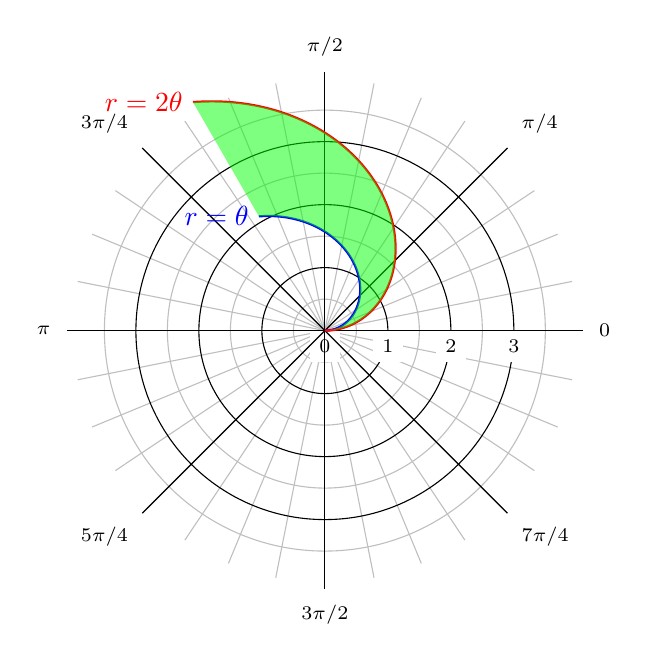
\begin{tikzpicture}[scale=.8, >=latex]

% Draw the lines at multiples of pi/12
\foreach \ang in {0,...,31} {
  \draw [lightgray] (0,0) -- (\ang * 180 / 16:4);
}

% Concentric circles and radius labels
\foreach \s in {0, 1, 2, 3} {
  \draw [lightgray] (0,0) circle (\s + 0.5);
  \draw (0,0) circle (\s);
  \node [fill=white] at (\s, 0) [below] {\scriptsize $\s$};
}

% Add the labels at multiples of pi/4
\foreach \ang/\lab/\dir in {
  0/0/right,
  1/{\pi/4}/{above right},
  2/{\pi/2}/above,
  3/{3\pi/4}/{above left},
  4/{\pi}/left,
  5/{5\pi/4}/{below left},
  7/{7\pi/4}/{below right},
  6/{3\pi/2}/below} {
  \draw (0,0) -- (\ang * 180 / 4:4.1);
  \node [fill=white] at (\ang * 180 / 4:4.2) [\dir] {\scriptsize $\lab$};
}

% Plot r = theta (0 to 2pi/3)
\draw [thick, color=blue, domain=0:120, samples=100, smooth]
  plot (xy polar cs:angle=\x, radius={\x/180*pi}) node[left] {$r = \theta$};

% Plot r = 2theta (0 to 2pi/3)
\draw [thick, color=red, domain=0:120, samples=100, smooth]
  plot (xy polar cs:angle=\x, radius={2*\x/180*pi}) node[left] {$r = 2\theta$};

% Shading between r=theta and r=2theta
\fill [fill=green, fill opacity=0.5, domain=0:120, samples=100, smooth]
  plot (xy polar cs:angle=\x, radius={2*\x/180*pi}) -- plot [smooth, samples=100, domain=120:0]
  (xy polar cs:angle=\x, radius={\x/180*pi}) -- cycle;

\end{tikzpicture}
\end{center}

\vspace{0.5cm}

\begin{definition}{Double Integral in Polar Coordinates}
    If \( f(x, y) \) is a continuous function on a radially simple domain \( R \), then the double integral of \( f \) over \( R \) in polar coordinates is given by
    \[\int \int_{R} f(x, y) \, dA = \int_{\alpha}^{\beta} \int_{r = r_1(\theta)}^{r = r_2(\theta)} f(r \cos(\theta), r \sin(\theta)) \, r \, dr \, d\theta \]
    Note the additional \(r\) term which is the result of the general change of variables formula.
\end{definition}

Consider an example: \[r = 2 - 2\sin(\theta)\]

\begin{align*}
  A &= \int_{0}^{2\pi} \int_{0}^{2 - 2\sin(\theta)} r \, dr \, d\theta \\
    &= \int_{0}^{2\pi} \left[ \frac{1}{2} r^2 \right]_{0}^{2 - 2\sin(\theta)} d\theta \\
    &= \int_{0}^{2\pi} \frac{1}{2} (2 - 2\sin(\theta))^2 \, d\theta \\
    &= \frac{1}{2} \int_{0}^{2\pi} (4 - 8\sin(\theta) + 4\sin^2(\theta)) \, d\theta \\
    &= \frac{1}{2} \left( \int_{0}^{2\pi} 4 \, d\theta - \int_{0}^{2\pi} 8\sin(\theta) \, d\theta + \int_{0}^{2\pi} 4\sin^2(\theta) \, d\theta \right) \\
    &= \frac{1}{2} \left( 4\theta \Big|_{0}^{2\pi} - 8(-\cos(\theta)) \Big|_{0}^{2\pi} + 4 \int_{0}^{2\pi} \sin^2(\theta) \, d\theta \right) \\
    &= \frac{1}{2} \left( 8\pi + 4 \int_{0}^{2\pi} \sin^2(\theta) \, d\theta \right) \\
    &= \frac{1}{2} \left( 8\pi + 4 \int_{0}^{2\pi} \frac{1 - \cos(2\theta)}{2} \, d\theta \right) \quad \text{(using the identity $\sin^2(\theta) = \frac{1 - \cos(2\theta)}{2}$)} \\
    &= \frac{1}{2} \left( 8\pi + 4\pi - \int_{0}^{2\pi} \cos(2\theta) \, d\theta \right) \\
    &= \frac{1}{2} \left( 12\pi - 0 \right) \quad \text{(since the integral of $\cos(2\theta)$ over a full period is 0)} \\
    &= 6\pi
\end{align*}


\begin{center}
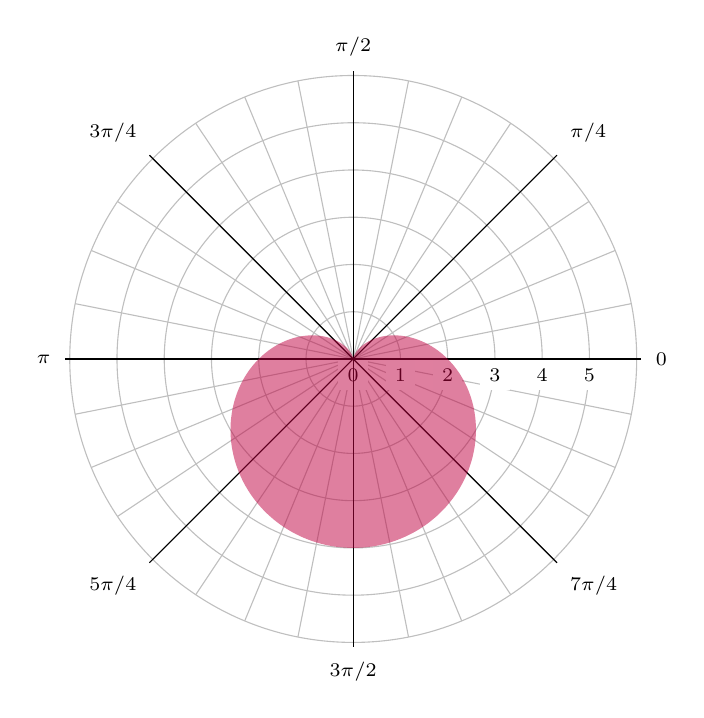
\begin{tikzpicture}[scale=0.6, >=latex]
% Draw the lines at multiples of pi/12
\foreach \ang in {0,...,31} {
  \draw [lightgray] (0,0) -- (\ang * 180 / 16:6);
}

% Concentric circles and radius labels
\foreach \s in {0, 1, 2, 3, 4, 5, 6} {
  \draw [lightgray] (0,0) circle (\s);
  \ifnum\s<6
    \node [fill=white] at (\s, 0) [below] {\scriptsize $\s$};
  \fi
}

% Add the labels at multiples of pi/4
\foreach \ang/\lab/\dir in {
  0/0/right,
  1/{\pi/4}/{above right},
  2/{\pi/2}/above,
  3/{3\pi/4}/{above left},
  4/{\pi}/left,
  5/{5\pi/4}/{below left},
  7/{7\pi/4}/{below right},
  6/{3\pi/2}/below} {
  \draw (0,0) -- (\ang * 180 / 4:6.1);
  \node [fill=white] at (\ang * 180 / 4:6.2) [\dir] {\scriptsize $\lab$};
}

% Plot and shade r = 2 - 2sin(theta) (0 to 2pi)
\fill [thick, color=purple, domain=0:360, samples=100, smooth, fill=purple, fill opacity=0.5]
  plot (xy polar cs:angle=\x, radius={2-2*sin(\x)});

\end{tikzpicture}
%\caption{Polar plot of \( r = 2 - 2\sin(\theta) \) with the region shaded in purple}
\end{center}


\begin{definition}{Rectangular to Cylindrical Coordinates}
    Given a point \( (x, y, z) \) in Euclidean coordinates, we can convert it to a point \( (r, \theta, z) \) in cylindrical coordinates by setting
    \[ z = z, \quad r = \sqrt{x^2 + y^2}, \quad \tan(\theta) = \frac{y}{x} \] (assuming \( x \neq 0 \)).
\end{definition}


\begin{definition}{Cylindrical to Rectangular Coordinates}
    Given a point \( (r, \theta, z) \) in cylindrical coordinates, we can convert it to a point \( (x, y, z) \) in rectangular coordinates by setting
    \[ x = r \cos(\theta), \quad y = r \sin(\theta), \quad z = z \]
\end{definition}


\begin{definition}{Rectangular to Spherical Coordinates}
    Given a point \( (x, y, z) \) in standard Euclidean coordinates, we can convert it to spherical coordinates by setting
    \[ \rho = \sqrt{x^2 + y^2 + z^2}, \quad \tan(\theta) = \frac{y}{x}, \quad \cos(\phi) = \frac{z}{\rho} \]
\end{definition}


\begin{definition}{Spherical to Rectangular Coordinates}
    Given a point \( (\rho, \theta, \phi) \) in spherical coordinates, we can convert it to standard Euclidean coordinates by setting
    \[ x = \rho \sin(\phi) \cos(\theta), \quad y = \rho \sin(\phi) \sin(\theta), \quad z = \rho \cos(\phi) \]
\end{definition}

\begin{definition}{Centrally Simple}
    A solid region \( R \subset \R^3 \) is called centrally simple if \( R \) is of the form 
    \[ R = \{(\rho, \theta, \phi) \mid \theta_1 \leq \theta \leq \theta_2, \, \phi_1 \leq \phi \leq \phi_2, \, \rho_1(\theta, \phi) \leq \rho \leq \rho_2(\theta, \phi)\} \]
\end{definition}

\begin{definition}{Triple Integrals in Spherical Coordinates}
    Let \( f(x, y, z) \) be a continuous function on a centrally simple region \( R \). Define 
    \[ g(\theta, \phi, \rho) = f(\rho \sin(\phi) \cos(\theta), \rho \sin(\phi) \sin(\theta), \rho \cos(\phi)) \]
    Then the integral of \( f \) over \( R \) is given by
    \[ \int \int \int_R f(x,y,z) \, dV = \int_{\theta_1}^{\theta_2} \int_{\phi_1}^{\phi_2} \int_{\rho = \rho_1(\theta,\phi)}^{\rho = \rho_2(\theta,\phi)} g(\theta, \phi, \rho) \, \rho^2 \sin(\phi) \, d\rho \, d\phi \, d\theta \]
    Like with double integrals in polar, there is an extra term \(\rho^2 \sin(\phi)\) from the general change of variables formula. 
\end{definition}


\section*{Linear Algebra Review}

\begin{definition}{Linear Maps}
    A linear map \( T:V \to W \) is defined as follows for all \( k \in \mathbb{N}, \alpha_{i} \in \R \), and all vectors \( \bm{x}_i \in V \):
    \[ T\left(\sum\limits_{i=1}^{k}\alpha_{i}\bm{x}_{i}\right) = \sum\limits_{i=1}^{k}\alpha_{i}T(\bm{x}_{i}) \]

    Equivalently, a linear map will satisfy the following:
    \begin{enumerate}
        \renewcommand{\labelenumi}{\roman{enumi}}
        \item \( T(\bm{u} + \bm{v}) = T(\bm{u}) + T(\bm{v}) \)
        \item \( T(\lambda \bm{u}) = \lambda T(\bm{u}) \)
    \end{enumerate}

    Additionally, a map \( T : \R^n \to \R^m \) is linear if and only if there is a matrix \( A \) in \( M_{m \times n}(\R) \) such that
    \[ T(\bm{x}) = A\bm{x} \]
    We call \( A \) the standard matrix of \( T \).
\end{definition}


\begin{definition}{Standard Matrix}
    Given a basis \( \mathcal{B} = \{ \bm{e_1}, \ldots, \bm{e_n} \} \), the standard matrix \( A \) of a linear map \( T: \R^n \to \R^m \) is given by 
    \[ \begin{bmatrix} A \end{bmatrix} = \begin{bmatrix}
    | & | & & | \\
    T(\bm{e_1}) & T(\bm{e_2}) & \cdots & T(\bm{e_n}) \\
    | & | & & |
    \end{bmatrix} \in M_{m \times n} (\R) \]
\end{definition}

\begin{definition}{Area of a Parallelogram}
    Let \( P \) be the parallelogram spanned by \( \bm{u} = \langle A, B \rangle \) and \( \bm{v} = \langle C, D \rangle \) in \( \R^2 \). 
    \[ \text{area}(P) = \left| \det\begin{bmatrix} A & B \\ C & D \end{bmatrix} \right| \]
    That is, the absolute value of a \( 2 \times 2 \) determinant equals the area of the parallelogram spanned by the rows.
\end{definition}

\begin{definition}{Volume of a Parallelepiped}
    Let \( D \) be the parallelepiped spanned by vectors \( \bm{u}, \bm{v}, \) and \( \bm{w} \) in \( \R^3 \). Then the volume of \( D \) is given by the absolute value of the scalar triple product:
    \[ \text{volume}(D) = |\bm{u} \cdot (\bm{v} \times \bm{w})| = \left| \det\begin{bmatrix} \bm{u} \\ \bm{v} \\ \bm{w} \end{bmatrix} \right| \]

    This generalizes in the following way. Let \( D \) be the parallelepiped spanned by vectors \( \bm{v_1}, \bm{v_2}, \ldots, \bm{v_n} \) in \( \R^n \). Then the n-dimensional volume of \( D \) is given by the absolute value of the determinant:
    \[ \text{vol}_n(D) = \left| \det\begin{bmatrix} \bm{v_1} \\ \vdots \\ \bm{v_n} \end{bmatrix} \right| \]
\end{definition}

\begin{definition}{Volume of a Region Under a Linear Transformation}
Let \( D \subset \R^n \) and \( T(\bm{x}) = A\bm{x} \) be a linear transformation. The volume of \( D \), \( \text{vol}_n(D) \), and the volume of the transformed region \( T(D) \) are related by:
\[
\text{vol}_n(T(D)) = \left| \det(A) \right| \text{vol}_n(D)
\]
where \( \det(A) \) is the determinant of \( A \).
\end{definition}

\noindent \textbf{Injective}

Let \( f: V \rightarrow W \) be a linear map. We say that \( f \) is injective or one-to-one (or sometimes, \( f \) is an injection) if the following holds:
For all \( \bm{v}_1, \bm{v}_2 \in V \), if \( f(\bm{v}_1) = f(\bm{v}_2) \), then \( \bm{v}_1 = \bm{v}_2 \).

That is, a map \( f \) is injective if any element in the codomain of \( f \) is the image of at most one element in its domain.

\begin{center}
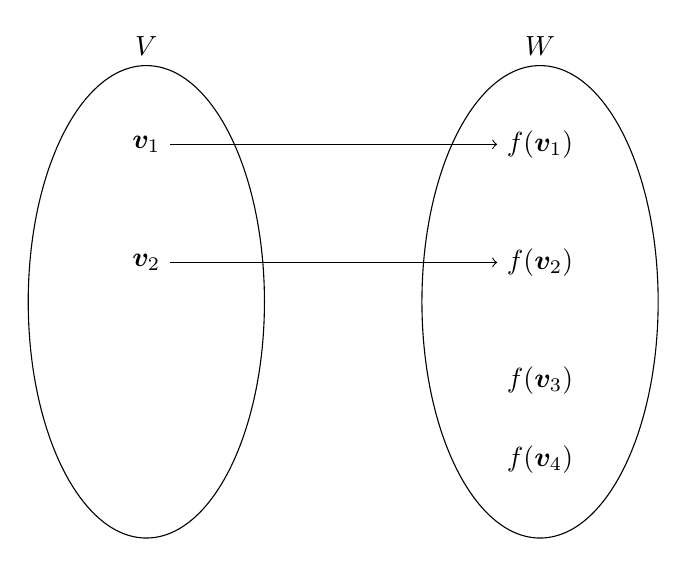
\begin{tikzpicture}
    % Draw the sets V and W
    \draw (0,0) ellipse (1.5cm and 3cm) node[above=3cm] {$V$};
    \draw (5,0) ellipse (1.5cm and 3cm) node[above=3cm] {$W$};

    % Nodes in V
    \node (v1) at (0,2) {$\bm{v}_1$};
    \node (v2) at (0,0.5) {$\bm{v}_2$};

    % Nodes in W
    \node (w1) at (5,2) {$f(\bm{v}_1)$};
    \node (w2) at (5,0.5) {$f(\bm{v}_2)$};
    \node (w3) at (5,-1) {$f(\bm{v}_3)$};
    \node (w4) at (5,-2) {$f(\bm{v}_4)$};

    % Arrows
    \draw[->] (v1) -- (w1);
    \draw[->] (v2) -- (w2);

\end{tikzpicture}
\end{center}

\vspace{0.5cm}

\section*{(Non-linear) Change of Variables}

\begin{definition}{The Jacobian}
Let \( f : A \subset \R^m \rightarrow \R^n \) be a multivariable function defined by \( f^i : A \subset \R^m \rightarrow \R \):
\[
f(\bm{x}) =
\begin{bmatrix}
    f^1(\bm{x}) \\
    \vdots \\
    f^n(\bm{x})
\end{bmatrix}.
\]
The Jacobian matrix of \( f \) at \( \bm{x}_0 \) is
\[
[J_f (\bm{x}_0)] =
\begin{bmatrix}
    D_1f^1(\bm{x}_0) & D_2f^1(\bm{x}_0) & \cdots & D_mf^1(\bm{x}_0) \\
    D_1f^2(\bm{x}_0) & D_2f^2(\bm{x}_0) & \cdots & D_mf^2(\bm{x}_0) \\
    \vdots & \vdots & \ddots & \vdots \\
    D_1f^n(\bm{x}_0) & D_2f^n(\bm{x}_0) & \cdots & D_mf^n(\bm{x}_0)
\end{bmatrix},
\]
if the partial derivatives exist.
\end{definition}


\begin{definition}{Determinant of the Jacobian}
    Given a differentiable map \( G(u,v) = (x(u,v),y(u,v)) \), the Jacobian matrix, denoted as \([J_G]\), is the matrix of partial derivatives:
    \[
    [J_G] = 
    \begin{bmatrix}
    \frac{\partial x}{\partial u} & \frac{\partial x}{\partial v} \\
    \frac{\partial y}{\partial u} & \frac{\partial y}{\partial v}
    \end{bmatrix}.
    \]
    The determinant of the Jacobian matrix is denoted as \(\text{Jac}(G)\). Thus,
    \[
    \det([J_G]) = \text{Jac}(G) = \frac{\partial x}{\partial u} \frac{\partial y}{\partial v} - \frac{\partial x}{\partial v} \frac{\partial y}{\partial u}.
    \]
\end{definition}

\begin{definition}{Approximation of the Volume of a Non-Linear Map}
Let \( D \subset \R^n \) be a region such that \( \text{vol}_n(D) \) is small, and let \( p \in D \). Let \( G : \R^n \rightarrow \R^n \) be a differentiable map. Then
\[
\text{vol}_n(G(D)) \approx \left| \det\left([J_G](p)\right) \right| \text{vol}_n(D).
\]
That is, the \( n \)-dimensional volume of \( G(D) \) can be approximated by the \( n \)-dimensional volume of \( [J_G](p)(D) \).
\end{definition}

\begin{definition}{Change of Variables}
Let \( K \subset \R^n \) be a compact set such that \( \text{vol}_n(\partial K) = 0 \). Let \( U \subset \R^n \) be an open set containing \( K \). Let
\( G : U \rightarrow \R^n \)
be a map such that:
\begin{enumerate}
    \item \( G \) is differentiable.
    \item \( G \) is injective on the interior of \( K \).
    \item \( \det([J_G]) \neq 0 \) on the interior of \( K \).
\end{enumerate}

Then, if \( f : G(K) \rightarrow \R \) is a continuous function, then
\[
\int_{G(K)} f \, dV = \int_{K} (f \circ G) \left| \det([J_G]) \right| \, dV.
\]

Sometimes, it is easier to consider a map in the reverse direction, denoted as
\[
F(\bm{x}, \bm{y}) = (u(x, y), v(x, y)).
\]

Then let \( G = F^{-1} \). If \( G = F^{-1} \) and \( \det([J_G]) \neq 0 \), then
\[
\det([J_G]) = \frac{1}{\det([J_F])}.
\]

\end{definition}

\begin{definition}{Example of Change of Variables - Volume of a Unit Sphere in \(\R^3\)}
Consider the volume of the unit sphere in \(\R^3\). The spherical coordinates transformation \( F \) maps from spherical coordinates \((\rho, \theta, \phi)\) to Cartesian coordinates \((x, y, z)\) and is given by:
\[
F(\rho, \theta, \phi) = 
\begin{bmatrix}
    \rho \sin(\phi) \cos(\theta) \\
    \rho \sin(\phi) \sin(\theta) \\
    \rho \cos(\phi)
\end{bmatrix}.
\]

The Jacobian matrix \( [J_F] \) of this transformation is:
\[
[J_F] = 
\begin{bmatrix}
    \sin(\phi)\cos(\theta) & -\rho\sin(\phi)\sin(\theta) & \rho\cos(\phi)\cos(\theta) \\
    \sin(\phi)\sin(\theta) & \rho\sin(\phi)\cos(\theta) & \rho\cos(\theta)\sin(\phi) \\
    \cos(\phi) & 0 & -\rho\sin(\phi)
\end{bmatrix}
\]


\begin{align*}
\det = \, & \cos(\phi) \cdot \det\begin{bmatrix}
    -\rho\sin(\phi)\sin(\theta) & \rho\cos(\phi)\cos(\theta) \\
    \rho\sin(\phi)\cos(\theta) & \rho\sin(\theta)\cos(\phi)
\end{bmatrix} \\
&- 0 \cdot \det\begin{bmatrix}
    \sin(\phi)\cos(\theta) & \rho\cos(\phi)\cos(\theta) \\
    \sin(\phi)\sin(\theta) & \rho\sin(\theta)\cos(\phi)
\end{bmatrix} \\
&+ (-\rho\sin(\phi)) \cdot \det\begin{bmatrix}
    \sin(\phi)\cos(\theta) & -\rho\sin(\phi)\sin(\theta) \\
    \sin(\phi)\sin(\theta) & \rho\sin(\phi)\cos(\theta)
\end{bmatrix} \\
= \, & \cos(\phi) \cdot \left( (-\rho\sin(\phi)\sin(\theta)) \cdot (\rho\sin(\theta)\cos(\phi)) - (\rho\cos(\phi)\cos(\theta)) \cdot (\rho\sin(\phi)\cos(\theta)) \right) \\
&+ \rho\sin(\phi) \cdot \left( (\sin(\phi)\cos(\theta)) \cdot (\rho\sin(\phi)\cos(\theta)) - (-\rho\sin(\phi)\sin(\theta)) \cdot (\sin(\phi)\sin(\theta)) \right) \\
= \, & \rho^2 \cos(\phi)\sin(\phi)\sin^2(\theta) - \rho^2 \cos^2(\phi)\cos(\theta)\sin(\phi) \\
&+ \rho^2 \sin(\phi)\cos(\theta)\sin^2(\phi) + \rho^2 \sin^3(\phi)\sin(\theta)\cos(\theta) \\
= \, & \rho^2 \sin(\phi) (\cos(\phi)\sin^2(\theta) - \cos^2(\phi)\cos(\theta) + \sin^2(\phi)\cos(\theta) + \sin^2(\theta)\cos(\theta)\sin(\phi)) \\
= \, & \rho^2 \sin(\phi) (\cos(\phi) - \cos^2(\phi) + \sin^2(\phi)) \\
= \, & -\rho^2 \sin(\phi).
\end{align*}


The determinant of the Jacobian matrix \( \det([J_F]) \) is:
\[
\det([J_F]) = -\rho^2 \sin(\theta).
\]

And we consider:

\[
\left|\det([J_F])\right| = \rho^2 \sin(\theta).
\]

To find the volume of the unit sphere, integrate \( \det([J_F]) \) over the appropriate bounds for \( \rho \), \( \theta \), and \( \phi \):
\[
\text{Volume} = \int_{0}^{2\pi} \int_{0}^{\pi} \int_{0}^{1} \rho^2 \sin(\theta) \, d\rho \, d\theta \, d\phi.
\]



\begin{align*}
\text{Volume} &= \int_{0}^{2\pi} \int_{0}^{\pi} \int_{0}^{1} r^2 \sin(\theta) \, d\rho \, d\theta \, d\phi \\
&= \int_{0}^{2\pi} \int_{0}^{\pi} \left[ \frac{1}{3}\rho^3 \right]_{0}^{1} \sin(\theta) \, d\theta \, d\phi \\
&= \int_{0}^{2\pi} \int_{0}^{\pi} \frac{1}{3} \sin(\theta) \, d\theta \, d\phi \\
&= \int_{0}^{2\pi} \left[ -\frac{1}{3} \cos(\theta) \right]_{0}^{\pi} \, d\phi \\
&= \int_{0}^{2\pi} \frac{2}{3} \, d\phi \\
&= \left[ \frac{2}{3} \phi \right]_{0}^{2\pi} \\
&= \frac{4\pi}{3}.
\end{align*}

\end{definition}

\begin{definition}{Volume of the Unit Ball in \(\R^4\) Using Spherical Coordinates}

The spherical coordinate system in \(\R^4\) extends the traditional system in \(\R^3\) by introducing an additional angle, leading to coordinates \((r, \psi, \theta, \phi)\). In this system, a point in \(\R^4\) is represented as:

\[
\begin{aligned}
x &= r \sin(\psi) \sin(\theta) \cos(\phi), \\
y &= r \sin(\psi) \sin(\theta) \sin(\phi), \\
z &= r \sin(\psi) \cos(\theta), \\
w &= r \cos(\psi),
\end{aligned}
\]

where \(0 \leq r \leq 1\), \(0 \leq \psi \leq \pi\), \(0 \leq \theta \leq \pi\), and \(0 \leq \phi \leq 2\pi\).

The volume of the unit ball in \(\R^4\) is computed using the integral:

\[
\text{Volume} = \int_{0}^{1} \int_{0}^{\pi} \int_{0}^{\pi} \int_{0}^{2\pi} \left| -r^3 \sin^2(\psi) \sin(\theta) \right| \, d\phi \, d\theta \, d\psi \, dr.
\]

Without delving into the specifics of the Jacobian determinant calculation, this setup directly leads to the volume of the unit ball in \(\R^4\) being \(\frac{\pi^2}{2}\).

\end{definition}


\hrulefill

\begin{center}
    \textit{Post Midterm 1 Material}
\end{center}

\section{Curves and Surfaces}

\begin{definition}{Surjective}
    A map $f : X \to Y$ is \textbf{surjective} if for every $\bm{y} \in Y$, there exists an $\bm{x} \in X$ such that $f(\bm{x}) = \bm{y}$.
    \end{definition}

\begin{definition}{Injective}
    A map \(f: X \to Y\) is \textbf{injective} if \(f(\bm{x_1}) = f(\bm{x_2}) \implies \bm{x_1} = \bm{x_2}\)
\end{definition}

\subsection{Curves}

\begin{definition}{Strict Parametrization}
A strict parametrization of a curve \( \mathcal{C} \subset \R^n \) is a vector-valued function \( \bm{r}(t) : (a, b) \subset \R \to \mathcal{C} \) satisfying the following conditions:
\begin{enumerate}
    \item \( \bm{r}(t) \) surjects onto \( \mathcal{C} \).
    \item \( \bm{r}(t) \) is injective for all \( t \in (a, b) \).
    \item \( \bm{r}(t) \) is differentiable.
    \item \( \bm{r}'(t) \neq 0 \) for all \( t \in (a, b) \).
\end{enumerate}
\end{definition}

\begin{definition}{Arclength}
Let \( C \) be a curve in \( \R^n \), and let \( \bm{r}(t) : (a, b) \to \R^n \) be a (strict) parametrization of \( C \).
Then the arclength of \( C \) is defined to be the integral
\[
\int_{a}^{b} \left\| \bm{r}'(t) \right\| \, dt
\]
\end{definition}

\begin{definition}{Scalar Line Integral}
Let \( f : \R^n \to \R \) be a function of \( n \) variables, and let \( \mathcal{C} \) be a curve in \( \R^n \). Let \( \bm{r}(t) : (a, b) \to \R^n \) be a (strict) parametrization of \( C \). Then the scalar line integral of \( f \) over \( \mathcal{C} \) is denoted \(\int_C f \, ds\), and is defined as the integral
\[
\int_{a}^{b} f(\bm{r}(t)) \left\| \bm{r}'(t) \right\| \, dt
\]
\end{definition}


\begin{definition}{Open Subset}
Let \(A \subset \mathbb{R}^n\). We say that \(A\) is an open subset of \(\mathbb{R}^n\) if \(A\) does not contain any of its boundary points. That is,
\[ A \cap \partial A = \varnothing \]
\end{definition}

\begin{definition}{Parameterization of a Curve (non-strict)}
Let \(\mathcal{C}\) be a curve in \(\mathbb{R}^n\). Let \(A \subset \mathbb{R}\) be a subset such that \(\text{vol}_1(\partial A) = 0\). Let \(X \subset A\) be a subset such that \(A - X\) is open. Then \(\gamma: A \to \mathbb{R}^n\) is a parametrization of \(\mathcal{C}\) if:
\begin{enumerate}
    \item \(\mathcal{C} \subset \gamma(A)\) (that is, \(\gamma\) surjects onto \(\mathcal{C}\)).
    \item \(\gamma(A - X) \subset \mathcal{C}\), and \(\gamma: A - X \to \mathcal{C}\) is injective.
    \item \(\gamma(t)\) is differentiable for all \(t \in A - X\).
    \item \(\gamma'(t) \neq \bm{0}\) for all \(t \in A - X\).
    \item \(\text{vol}_1(X) = 0\).
\end{enumerate}
\end{definition}



\subsection{Surfaces}

\begin{definition}{Strict Parameterization of a Surface}
A strict parametrization of a surface \(\mathcal{S} \subset \mathbb{R}^3\) is a multivariable function \(G(u, v) : U \subset \mathbb{R}^2 \to \mathcal{S}\) satisfying the following conditions:
\begin{enumerate}
    \item \(U\) is an open set.
    \item \(G(u, v)\) surjects onto \(\mathcal{S}\).
    \item \(G(u, v)\) is injective for all \(\bm{u} \in U\).
    \item \(G(u, v)\) is differentiable for all \(\bm{u} \in U\) (that is, \(\partial G/\partial u\) and \(\partial G/\partial v\) exist).
    \item The Jacobian matrix \([J_G(u, v)]\) is injective (i.e., has full rank) for all \(\bm{u} \in U\).
\end{enumerate}
\end{definition}


\begin{definition}{Useful Statements on Injectivity}
The following statements are equivalent about a linear transformation \(T : \mathbb{R}^n \to \mathbb{R}^m\) with standard matrix \(A\):
\begin{enumerate}
    \item \(T\) is injective.
    \item The only solution to the equation \(A\bm{x} = \bm{0}\) is \(\bm{x} = \bm{0}\).
    \item If the equation \(A\bm{x} = \bm{b}\) has a solution, it is unique.
    \item The columns of \(A\) are linearly independent.
\end{enumerate}
\end{definition}

\begin{definition}{Tangent Plane to Surface}
The tangent plane to a surface \(S\) at a point \(G(u_0, v_0)\) is spanned by the vectors
\[
\frac{\partial G}{\partial u}(u_0, v_0) = \left( \frac{\partial x}{\partial u}(u_0, v_0), \frac{\partial y}{\partial u}(u_0, v_0), \frac{\partial z}{\partial u}(u_0, v_0) \right)
\]
and
\[
\frac{\partial G}{\partial v}(u_0, v_0) = \left( \frac{\partial x}{\partial v}(u_0, v_0), \frac{\partial y}{\partial v}(u_0, v_0), \frac{\partial z}{\partial v}(u_0, v_0) \right).
\]
\end{definition}

\begin{definition}{Parameterization of a Surface (non-strict)}
Let \(\mathcal{S} \subset \mathbb{R}^3\) be a surface. Let \(A \subset \mathbb{R}^2\) be a subset such that \(\text{vol}_2(\partial A) = 0\). Let \(X \subset A\) be a subset such that \(A - X\) is open. Then a map \(\gamma : A \to \mathbb{R}^3\) parametrizes \(\mathcal{S}\) if:
\begin{enumerate}
    \item \(\mathcal{S} \subset \gamma(A)\) (that is, \(\gamma\) surjects onto \(\mathcal{S}\)).
    \item \(\gamma(A - X) \subset \mathcal{S}\), and \(\gamma : A - X \to \mathcal{S}\) is injective.
    \item \(\gamma\) is differentiable for all \(\bm{u} \in A - X\).
    \item \([J_{\gamma}(\bm{u})]\) is injective for all \(\bm{u} \in A - X\).
    \item \(\text{vol}_2(X) = 0\) and for any compact subset \(\mathcal{C} \subset \mathcal{S}\), \(\text{vol}_2(\gamma(X) \cap \mathcal{C}) = 0\).
\end{enumerate}
\end{definition}

\begin{definition}{k-Dimensional Volume Zero}
Let \(X \subset \R^n\) be a bounded subset. We say that \(X\) has k-dimensional volume \(0\) (\(\text{vol}_k(X) = 0\)) if 
\[
\lim_{N \to \infty} \sum_{\substack{C \in D_N(\R^n) \\ C \cap X \neq \varnothing}} \left(\frac{1}{2^N}\right)^k = 0.
\]
Furthermore, now let \( X \subset \R^n \) be an arbitrary subset. We say that \(X\) has k-dimensional volume \(0\) if for all \(R > 0\), the intersection \(B_R(\bm{0}) \cap X\) has volume \(0\), where \(B_R(\bm{0})\) denotes the ball of radius \(R\) centered at the origin in \(\R^n\).
\end{definition}

\begin{definition}{Surface Area Integral}
Let \(\mathcal{S}\) be a surface (strictly) parametrized by a function \(\gamma : U \subset \R^2 \to \R^3\). Then the surface area of \(\mathcal{S}\) is given by
\[
\int_{\mathcal{S}} d\mathcal{S} = \int_{U} \left\| \frac{\partial \gamma}{\partial u} \times \frac{\partial \gamma}{\partial v} \right\| \, du \, dv,
\]
where \(\frac{\partial \gamma}{\partial u}\) and \(\frac{\partial \gamma}{\partial v}\) are the partial derivatives of \(\gamma\) with respect to \(u\) and \(v\), respectively, and \(\times\) denotes the cross product.
\end{definition}


\section{Manifolds}

\begin{definition}{K-Dimensional Manifold as the Graph of a Function}
A subset \(\mathcal{M} \subset \R^n\) is a differentiable k-dimensional manifold embedded in \(\R^n\) if, for all \(\bm{x} \in \mathcal{M}\), there exists an open neighborhood \(U \subset \R^n\) such that \(\mathcal{M} \cap U\) is the graph of a \(C^1\) mapping \(f : \R^k \to \R^{n-k}\).
\end{definition}

\begin{definition}{Parameterization of a Manifold}
Let \(\mathcal{M} \subset \R^n\) be a \(k\)-dimensional manifold embedded in \(\R^n\). Let \(A \subset \R^k\) be a subset such that \(\text{vol}_k(\partial A) = 0\). Let \(X \subset A\) be a subset such that \(A - X\) is open. Then a map \(\gamma : A \to \R^n\) parametrizes \(\mathcal{M}\) if:
\begin{enumerate}
    \item[(a)] \(\mathcal{M} \subset \gamma(A)\) (that is, \(\gamma\) surjects onto \(\mathcal{M}\)).
    \item[(b)] \(\gamma(A - X) \subset \mathcal{M}\), and \(\gamma : A - X \to \mathcal{M}\) is injective.
    \item[(c)] \(\gamma\) is differentiable for all \(\bm{u} \in A - X\).
    \item[(d)] \([J_\gamma(\bm{u})]\) is injective for all \(\bm{u} \in A - X\).
    \item[(e)] \(\text{vol}_k(X) = 0\) and for any compact subset \(\mathcal{C} \subset \mathcal{M}\), \(\text{vol}_k(\gamma(X) \cap \mathcal{C}) = 0\).
\end{enumerate}
\end{definition}

\begin{definition}{Differentiable Manifold and Tangent Space}
Let \(M \subset \R^n\) be a differentiable \(k\)-dimensional manifold. Consider a neighborhood \(U\) of a point \(\bm{z}_0 = (\bm{x}_0, \bm{y}_0) \in M\) such that the intersection of \(M\) and \(U\) can be represented as:
\[
M \cap U = \left\{ (\bm{x}, f(\bm{x})) \mid \bm{x} \in \R^k \right\},
\]
where \(f: \R^k \to \R^{n-k}\) is a differentiable function that locally describes \(M\) in the neighborhood of \(\bm{z}_0\).

The \textbf{tangent space} to \(M\) at \(\bm{z}_0\), denoted \(T_{\bm{z}_0}M\), is defined as the graph of the derivative of \(f\) at \(\bm{x}_0\), denoted \([J_f(\bm{x}_0)]\). This derivative, also known as the Jacobian matrix of \(f\) at \(\bm{x}_0\), maps directions in the input space \(\R^k\) to directions in the output space \(\R^{n-k}\), effectively describing how the manifold \(M\) changes direction at the point \(\bm{z}_0\). Mathematically, the tangent space can be expressed as:
\[
T_{\bm{z}_0}M = \left\{ (\bm{x}, [J_f(\bm{x}_0)](\bm{x})) \mid \bm{x} \in \R^k \right\}.
\]

The \textbf{tangent space} to a manifold described by a parameterization is defined as

\[
T\gamma(\bm{u})M = \text{Im}[J\gamma(\bm{u})]
\]
That is, the tangent space \(T\gamma(\bm{u})M\) at \(\bm{u}\) can be expressed as the image of the Jacobian matrix of \(\varphi\) at \(\bm{u}\), which maps vectors from \(\R^k\) into \(\R^n\). Mathematically, this is represented as:
\[
T\gamma(\bm{u})M = \left\{ [J\gamma(\bm{u})](\bm{x}) \in \R^n \mid \bm{x} \in \R^k \right\}.
\]

\end{definition}


\begin{definition}{Volume of a \(k\)-Dimensional Parallelepiped in \(\R^k\)}
Let \(D\) be the \(k\)-dimensional parallelepiped spanned by \(\bm{v}_1, \ldots, \bm{v}_k\) in \(\R^k\). Consider the \(k \times k\) matrix \(T\) given by the vectors \(\bm{v}_1, \ldots, \bm{v}_k\) as columns. Then, the volume of \(D\) is given by
\[
\text{volume}(D) = |\det(T)| = \sqrt{\det(T^\top T)},
\]
where \(T^\top\) denotes the transpose of \(T\).
\end{definition}


\begin{definition}{Volume of a \(k\)-Dimensional Parallelepiped in \(\R^k\) and \(\R^n\)}
Let \(D\) be the \(k\)-dimensional parallelepiped spanned by \(\bm{v}_1, \ldots, \bm{v}_k\) in \(\R^k\). Consider the \(k \times k\) matrix \(T\) given by the vectors \(\bm{v}_1, \ldots, \bm{v}_k\) as columns. Then, the volume of \(D\) in \(\R^k\) is given by
\[
\text{volume}(D) = |\det(T)| = \sqrt{\det(T^\top T)},
\]
where \(T^\top\) denotes the transpose of \(T\).

\vspace{0.7cm}
Furthermore, now let \(D\) be the \(k\)-dimensional parallelepiped spanned by \(\bm{v}_1, \ldots, \bm{v}_k\) in \(\R^n\). While the \(\det(T)\) is meaningless in this context, we have 
\[
\text{volume}(D) = \sqrt{\det(T^\top T)},
\]
meaning the \(k\)-dimensional volume in \(\R^n\).
\end{definition}

\begin{definition}{Integral Over a Manifold}
Let \(\mathcal{M} \subset \R^n\) be a differentiable \(k\)-dimensional manifold, let \(A \subset \R^k\) be a set with well-defined volume, and let \(\gamma : A \to \R^n\) be a parametrization of \(\mathcal{M}\). Let \(f : \R^n \to \R\) be a function. We say \(f\) is integrable over \(\mathcal{M}\) if the following integral exists and is well-defined:
\[
\int_{\mathcal{M}} f \, d\mathcal{M} = \int_{A} f(\gamma(\bm{u})) \sqrt{ \det\left([J_\gamma(\bm{u})]^\top [J_\gamma(\bm{u})]\right)} \, d\bm{u},
\]
\end{definition}

\begin{definition}{Useful Statements on Surjectivity}
The following statements are equivalent about a linear transformation \(T : \R^n \to \R^m\) with standard matrix \(A\):
\begin{enumerate}
    \item[(a)] \(T\) is surjective.
    \item[(b)] The columns of \(A\) span \(\R^m\).
    \item[(c)] For every \(\bm{b} \in \R^m\), there exists \(\bm{x} \in \R^n\) such that \(A\bm{x} = \bm{b}\).
    \item[(d)] The rows of \(A\) are linearly indepedent.
\end{enumerate}
\end{definition}


\subsection{Manifolds as Vanishing Loci}

\begin{definition}{Vanishing Locus of a Function}
Let \(f : X \subset \R^n \to \R^m\) be a function. The vanishing locus of \(f\) (sometimes called the locus, or the zero locus) is the set of points \(V(f)\) where \(f\) vanishes. That is,
\[
V(f) = \{\bm{x} \in X \mid f(\bm{x}) = 0\}.
\]
\end{definition}


 \begin{definition}{Locally showing a vanishing locus is a differentiable manifold}
     Let $M$ be a subset of $\R^n$. Let $U \subset \R^n$ be open, and let $F : U \to \R^{n-k}$ be a $C^1$-mapping such that
    $$M \cap U = \{\bm{z} \in U \ | \ F(\bm{z}) = \bm{0} \}$$
    
    If the derivative $[J_F(\bm{z})]$ is a surjective map for every $\bm{z} \in M \cap U$, then $X \cap U$ is a differentiable $k$-dimensional manifold embedded in $\R^n$.  
\end{definition}


\begin{definition}{Showing a vanishing locus is a differentiable manifold}
    Let $M$ be a subset of $\R^n$.  If for every $\bm{z} \in M$, there exists an open set $U  \subset \R^n$ containing $\bm{z}$, and a $C^1$-mapping $F : U \subset \R^n \to \R^{n-k}$ such that 
    $$M \cap U = \{\bm{z} \in U \ | \ F(\bm{z}) = \bm{0} \}$$
    and $[J_F(\bm{z})]$ is surjective for every $\bm{z} \in M$, then $M$ is a differentiable $k$-dimensional manifold.
\end{definition}

    \begin{definition}{A differentiable manifold is locally a vanishing locus}
    Let $M \subset \R^n$ be differentiable $k$-dimensional manifold.  Then every point $\bm{z} \in M$ has a neighborhood $U \subset \R^n$ such that there exists a $C^1$-mapping $F : U \to \R^{n-k}$ such that $[J_F(\bm{z})]$ is surjective, and
    $$M \cap U = \{\bm{z} \in U \ | \ F(\bm{z}) = \bm{0} \}$$
    
    \end{definition}


\begin{definition}{Inverse Image of a Manifold Theorem}
Let \( M \subset \R^m \) be a differentiable \( k \)-dimensional manifold embedded in \( \R^m \). Let \( U \subset \R^n \), and let \( f: U \to \R^m \) be a \( C^1 \)-mapping. Define \( f^{-1}(M) \) to be the inverse image of \( M \),
\[ f^{-1}(M) = \{ \bm{x} \in \R^n \mid f(\bm{x}) \in M \} \]
If the derivative \( [J_f(\bm{x})] \) is a surjective map for every \( \bm{x} \in f^{-1}(M) \) in \( \R^n \), then \( f^{-1}(M) \) is a differentiable \( k + n - m \)-dimensional manifold embedded in \( \R^n \).
\end{definition}

\begin{definition}{Independence of Coordinates Corollary}
Let \( g: \R^n \to \R^n \) be a mapping of the form
\[ g(\bm{x}) = A\bm{x} + \bm{c} \]
where \( A \in M_{n \times n}(\R) \) is an invertible \( n \times n \) matrix. If \( M \) is a differentiable \( k \)-dimensional manifold, then \( g(M) \) is also a differentiable \( k \)-dimensional manifold.
\end{definition}


\section{Vector Fields}

\begin{definition}{Conservative Vector Field}
A vector field \(\bm{F} : \R^n \to \R^n\) is called conservative if there exists a differentiable function \(f(x_1, \ldots, x_n)\) such that
\[\bm{F} = \nabla f = \left\langle \frac{\partial f}{\partial x_1}, \ldots, \frac{\partial f}{\partial x_n} \right\rangle.\]
The function \(f\) is called a potential function for \(\bm{F}\).
\end{definition}


\begin{definition}{Divergence}
Given a vector field \(\bm{F} : \R^n \rightarrow \R^n\) defined by \(\bm{F}(\bm{u}) = \langle F_1(\bm{u}), \ldots, F_n(\bm{u}) \rangle\), the divergence of \(\bm{F}\) is the scalar-valued function div\(\bm{F} : \R^n \rightarrow \R\) defined by
\[ \text{div}\bm{F}(\bm{u}) = \frac{\partial F_1}{\partial x_1}(\bm{u}) + \cdots + \frac{\partial F_n}{\partial x_n}(\bm{u}). \]
In operator notation, this is written as
\[ \text{div}\bm{F} = \nabla \cdot \bm{F} = \left\langle \frac{\partial}{\partial x_1}, \ldots, \frac{\partial}{\partial x_n} \right\rangle \cdot \bm{F}. \]

The divergence of a vector field at a point \(P\) measures the net flux of \(\bm{F}\) out of an infinitesimally small sphere centered at \(P\). It characterizes the behavior of the vector field at \(P\) as follows:
\begin{itemize}
    \item If \(\text{div}\bm{F}(P) > 0\), then \(P\) is a source.
    \item If \(\text{div}\bm{F}(P) < 0\), then \(P\) is a sink.
    \item If \(\text{div}\bm{F}(P) = 0\), then \(P\) is said to be incompressible.
\end{itemize}
\end{definition}

\begin{definition}{Curl}
Given a vector field in \(\R^3\), \(\bm{F} = \langle F_1, F_2, F_3 \rangle\), the curl of \(\bm{F}\) is the vector field defined by
\[ \text{curl}\bm{F} = \left\langle \frac{\partial F_3}{\partial y} - \frac{\partial F_2}{\partial z}, \frac{\partial F_1}{\partial z} - \frac{\partial F_3}{\partial x}, \frac{\partial F_2}{\partial x} - \frac{\partial F_1}{\partial y} \right\rangle. \]
In operator notation, this can be written as
\[ \text{curl}\bm{F} = \nabla \times \bm{F} = \left\langle \frac{\partial}{\partial x}, \frac{\partial}{\partial y}, \frac{\partial}{\partial z} \right\rangle \times \bm{F}. \]
\end{definition}

\begin{definition}{Orientation of a Curve}
Given a curve \(\mathcal{C}\), a continuous choice of tangent vector on \(\mathcal{C}\) is called an orientation. A curve with a chosen orientation is called an oriented curve. Moving along the chosen direction is called the positive direction along \(\mathcal{C}\), and moving against the chosen orientation is called the negative direction (along \(\mathcal{C}\).

Given an oriented curve \(\mathcal{C}\) in \(\R^2\), we say that the positive direction across \(\mathcal{C}\) is the direction that goes left to right from the perspective of the positive orientation along \(\mathcal{C}\). Let \(\bm{n}(p)\) denote the unit vector normal to \(\mathcal{C}\) at the point \(p\), pointing in the positive direction across \(\mathcal{C}\).
\end{definition}



\begin{definition}{Vector Line Integral}
The line integral of a vector field \(\bm{F}\) along an oriented curve \(\mathcal{C}\) is denoted
\[ \int_{\mathcal{C}} \bm{F} \cdot d\bm{r}. \]
We define it as the integral of the tangential component of \(\bm{F}\) over \(\mathcal{C}\). Formally,
\[ \int_{\mathcal{C}} \bm{F} \cdot d\bm{r} := \int_{\mathcal{C}} (\bm{F} \cdot \bm{T}) \, ds \]
where \(\bm{T}\) is the unit tangent vector to \(\mathcal{C}\), and \(ds\) represents a differential element of arc length along \(\mathcal{C}\).

Let \(\bm{r}(t)\) be a positively oriented regular parametrization of an oriented curve \(\mathcal{C}\) for \(a \leq t \leq b\). Then the line integral of \(\bm{F}\) along \(\mathcal{C}\) can be computed as
\[ \int_{\mathcal{C}} \bm{F} \cdot d\bm{r} = \int_a^b \bm{F}(\bm{r}(t)) \cdot \bm{r}'(t) \, dt. \]

If \(\bm{F} = \langle F_1, F_2, F_3 \rangle\), then another common notation for line integrals is
\[ \int_{\mathcal{C}} \bm{F} \cdot d\bm{r} = \int_{\mathcal{C}} F_1 \, dx + F_2 \, dy + F_3 \, dz. \]
\end{definition}


\begin{definition}{Properties of Vector Line Integrals}
Let \(\mathcal{C}\) be a smooth oriented curve, and let \(\bm{F}\) and \(\bm{G}\) be vector fields.

\textbf{1. Linearity:}
\begin{itemize}
    \item The line integral is linear with respect to vector fields:
    \[ \int_{\mathcal{C}} (\bm{F} + \bm{G}) \cdot d\bm{r} = \int_{\mathcal{C}} \bm{F} \cdot d\bm{r} + \int_{\mathcal{C}} \bm{G} \cdot d\bm{r}. \]
    \item The line integral respects scalar multiplication:
    \[ \int_{\mathcal{C}} c\bm{F} \cdot d\bm{r} = c \int_{\mathcal{C}} \bm{F} \cdot d\bm{r}. \]
\end{itemize}

\textbf{2. Additivity:}
\begin{itemize}
    \item If \(\mathcal{C}\) is the union of smooth curves \(\mathcal{C}_1, \ldots, \mathcal{C}_n\), then
    \[ \int_{\mathcal{C}} \bm{F} \cdot d\bm{r} = \int_{\mathcal{C}_1} \bm{F} \cdot d\bm{r} + \cdots + \int_{\mathcal{C}_n} \bm{F} \cdot d\bm{r}. \]
\end{itemize}

\textbf{3. Reversing Orientation:}
\begin{itemize}
    \item If the orientation of \(\mathcal{C}\) is reversed, denoted as \(-\mathcal{C}\), then
    \[ \int_{-\mathcal{C}} \bm{F} \cdot d\bm{r} = -\int_{\mathcal{C}} \bm{F} \cdot d\bm{r}. \]
\end{itemize}
\end{definition}

\begin{definition}{Fundamental Theorem of Conservative Vector Fields}
Let \(\bm{F} = \nabla f\) be a conservative vector field on a domain \(D\). If \(\bm{r}\) is a path along a curve \(\mathcal{C}\) from point \(P\) to \(Q\) in \(D\), then
\[ \int_{\mathcal{C}} \bm{F} \cdot d\bm{r} = f(Q) - f(P). \]
In particular, this implies that \(\bm{F}\) is path-independent.

\textbf{Corollary:}
Let \(\bm{F} = \nabla f\) be a conservative vector field on a domain \(D\). If \(\bm{r}\) is a path along a closed curve \(\mathcal{C}\) in \(D\), then the circulation is zero:
\[ \oint_{\mathcal{C}} \bm{F} \cdot d\bm{r} = 0. \]
\end{definition}

\begin{definition}{Simply Connected}
A simply connected domain is a path-connected domain where one can continuously shrink any simple closed curve into a point while remaining within the domain. For two-dimensional regions, a simply connected domain is one without holes. For three-dimensional domains, the concept of simply connected is more subtle; it refers to a domain without any holes going all the way through it.
\end{definition}

\begin{definition}{From Zero Curl to Conservative}
Let \(\bm{F}\) be a vector field on a simply-connected domain \(D\). If \(\bm{F}\) satisfies the cross-partials condition (that is, the curl of \(\bm{F}\) is zero), then \(\bm{F}\) is conservative.
\end{definition}

\begin{definition}{Path Independence}
A vector field \(\bm{F}\) on a domain \(D\) is path-independent if for any two points \(P, Q \in D\), then
\[ \int_{\mathcal{C}_1} \bm{F} \cdot d\bm{r} = \int_{\mathcal{C}_2} \bm{F} \cdot d\bm{r} \]
for any two paths \(\mathcal{C}_1, \mathcal{C}_2\) in \(D\) that start at \(P\) and end at \(Q\).
\end{definition}

\begin{definition}{Normal Vector to Curve}
Let \(\bm{r}(t) = \langle x(t), y(t) \rangle\) be a positively oriented parametrization of an oriented curve \(\mathcal{C}\). Observe that \(\bm{N}(t) = \langle y'(t), -x'(t) \rangle\) is normal to \(\mathcal{C}\). Therefore, the unit normal vector \(\bm{n}(t)\) at any point on \(\mathcal{C}\) is given by
\[ \bm{n}(t) = \frac{\bm{N}(t)}{\|\bm{N}(t)\|}. \]
\end{definition}

\begin{definition}{Vector Flux Integral}
The flux integral of a vector field \(\bm{F}\) along an oriented curve \(\mathcal{C}\) in \(\R^2\) is the integral of the normal component of \(\bm{F}\):
\[ \int_{\mathcal{C}} \bm{F} \cdot \bm{n} \, ds. \]

Let \(\bm{r}(t) = \langle x(t), y(t) \rangle\) be a positively oriented parametrization of an oriented curve \(\mathcal{C}\) for \(a \leq t \leq b\). Then the flux integral of \(\bm{F}\) along \(\mathcal{C}\) can be computed as
\[ \int_{\mathcal{C}} \bm{F} \cdot \bm{n} \, ds = \int_{a}^{b} \bm{F}(\bm{r}(t)) \cdot \bm{N}(t) \, dt. \]
\end{definition}

\begin{definition}{Surface Orientation}
Given a surface \( \mathcal{S} \subset \R^3 \), a continuous choice of unit normal vector on \( \mathcal{S} \) is called an orientation. A surface with a chosen orientation is called an oriented surface.

Recall that given a parametrization \( \bm{G}(u, v) \) of \( \mathcal{S} \), then the normal vector at a point \( P = \bm{G}(u_0, v_0) \) on \( \mathcal{S} \) is determined by
\[ \bm{N}(P) = \frac{\partial \bm{G}}{\partial u}(u_0, v_0) \times \frac{\partial \bm{G}}{\partial v}(u_0, v_0). \]

Given an oriented surface, we say that a parametrization is positively oriented if the orientation given by
\[ \frac{\bm{N}(P)}{\|\bm{N}(P)\|} \]
agrees with the orientation of \( \mathcal{S} \).

If \( \bm{G}(u, v) \) is a strict parametrization of \( \mathcal{S} \), then the Jacobian matrix \( [J_{\bm{G}}(u, v)] \) is injective. Hence, \( \frac{\partial \bm{G}}{\partial u}(u_0, v_0) \) and \( \frac{\partial \bm{G}}{\partial v}(u_0, v_0) \) are linearly independent, so \( \bm{N}(P) \neq \bm{0} \). Otherwise, we have to worry about singularities in \( \mathcal{S} \).
\end{definition}

\begin{definition}{Vector Surface Integral}
The vector surface integral of \(\bm{F}\) over \(\mathcal{S}\) is defined as
\[ \iint_{\mathcal{S}} \bm{F} \cdot d\mathcal{S} := \iint_{\mathcal{S}} (\bm{F} \cdot \bm{n}) \, d\mathcal{S}. \]
This is also known as the flux of \(\bm{F}\) across (or through) \(\mathcal{S}\).

Let \(\bm{G}(u, v) : A \subseteq \R^2 \rightarrow \R^3\) be an oriented parametrization of a surface \(\mathcal{S}\). Then the vector surface integral can be computed as
\[ \iint_{\mathcal{S}} (\bm{F} \cdot \bm{n}) \, d\mathcal{S} = \iint_{A-X} \bm{F} (\bm{G}(u, v)) \cdot \bm{N}(u, v) \, du \, dv, \]
where \(\bm{N}(u, v)\) is the normal vector at the point \((u, v)\) on the parametrization domain \(A\), ensuring the orientation matches that of \(\mathcal{S}\).
\end{definition}

\begin{definition}{Flipped Orientation}
If \(-\mathcal{S}\) denotes \(\mathcal{S}\) with the opposite orientation, then the vector surface integral with the flipped orientation is given by
\[ \iint_{-\mathcal{S}} (\bm{F} \cdot \bm{n}) \, d\mathcal{S} = -\iint_{\mathcal{S}} (\bm{F} \cdot \bm{n}) \, d\mathcal{S}. \]
\end{definition}

\begin{definition}{Simple Closed Curve}
A simple closed curve \(\mathcal{C}\) is a closed curve that does not intersect itself.

\textit{Note: }A simple closed curve \(\mathcal{C}\) in \(\R^3\) can be thought of as the boundary of a surface \(\mathcal{S}\) in \(\R^3\).
\end{definition}


\begin{definition}{Jordan Curve Theorem}
A simple closed curve \(\mathcal{C}\) in \(\R^2\) splits \(\R^2\) into exactly two regions: an interior region \(D\), and the exterior region \(\R^2 - D\).
\end{definition}






\section{Green's theorem, Stokes' theorem, and the Divergence theorem}


\begin{definition}{Green's Theorem}
Let \(D\) be a region in \(\R^2\) such that \(\partial D\) is a disjoint union of simple closed curves, with \(\partial D\) oriented so that \(D\) is always to the left. Suppose \(\bm{F} = \langle F_1, F_2 \rangle\) is a smooth vector field on \(D\). Then
\[ \oint_{\partial D} \bm{F} \cdot d\bm{r} = \iint_{D} \left( \frac{\partial F_2}{\partial x} - \frac{\partial F_1}{\partial y} \right) dA. \]
\end{definition}

\begin{definition}{Green's Theorem in Circulation Form}
Let \(D\) be a region in \(\R^2\) such that \(\partial D\) is a simple closed curve, oriented counterclockwise. Suppose \(\bm{F} = \langle F_1, F_2 \rangle\) is a smooth vector field on \(D\). Then
\[ \oint_{\partial D} \bm{F} \cdot d\bm{r} = \iint_{D} \text{curl}_z (\bm{F}) \, dA. \]
\end{definition}

\begin{definition}{Green's Theorem in Flux Form}
Let \(D\) be a region in \(\R^2\) such that \(\partial D\) is a simple closed curve, oriented counterclockwise. Suppose \(\bm{F} = \langle F_1, F_2 \rangle\) is a smooth vector field on \(D\). Then
\[ \oint_{\partial D} \bm{F} \cdot \bm{n} \, ds = \iint_{D} \text{div}(\bm{F}) \, dA. \]
\end{definition}



\begin{definition}{Additivity of Circulation}
Let \(D\) be a region in \(\R^2\) such that \(\partial D\) is a simple closed curve, oriented counterclockwise. If we decompose a domain \(D\) into two domains \(D_1\) and \(D_2\) which intersect only on their boundaries, \(\partial D_1\) and \(\partial D_2\), then
\[ \oint_{\partial D} \bm{F} \cdot d\bm{r} = \oint_{\partial D_1} \bm{F} \cdot d\bm{r} + \oint_{\partial D_2} \bm{F} \cdot d\bm{r}. \]
\end{definition}


\begin{definition}{Upper Half Space}
The upper half-space \(H_k \subset \R^k\) is the (closed) set
\[ H_k := \{\bm{x} = \langle x_1, \ldots, x_k \rangle \mid x_k \geq 0\}. \]
This is a \(k\)-dimensional manifold with boundary
\[ \partial H_k = \{\langle x_1, \ldots, x_k \rangle \mid x_k = 0\}. \]
\end{definition}

\begin{definition}{Manifold with Boundary}
A subset \(\mathcal{M} \subset \R^n\) is a differentiable \(k\)-dimensional manifold with boundary embedded in \(\R^n\) if for all \(\bm{z} \in \mathcal{M}\), either:
\begin{enumerate}
    \item There exists an open neighborhood \(U \subset \R^n\) such that there exists a \(C^1\)-mapping \(F : U \rightarrow \R^{n-k}\) such that
    \begin{itemize}
        \item \(\mathcal{M} \cap U = \{\bm{z} \in U \mid F(\bm{z}) = \bm{0}\}\)
        \item \([J_F(\bm{z})]\) is surjective.
    \end{itemize}
    \item Or, there exists an open neighborhood \(V \subset \R^n\) such that there exists a \(C^1\)-mapping \(G : V \rightarrow \R^{m+n-k}\) such that
    \begin{itemize}
        \item \(G(\bm{x}) = \langle F_1(\bm{x}), F_2(\bm{x}) \rangle\)
        \item \(F_1 : V \rightarrow \R^{n-k}\), and \(F_2 : V \rightarrow \R^m\)
        \item \(G(\bm{z}) = \bm{0}\)
        \item \(\mathcal{M} \cap V = \{\bm{x} \in V \mid F_1(\bm{x}) = \bm{0}, F_2(\bm{x}) \geq 0\}\)
        \item \([J_G(\bm{z})]\) is surjective.
    \end{itemize}
\end{enumerate}
We say that the set of points \(\bm{z} \in \mathcal{M}\) satisfying the latter condition are the boundary of \(\mathcal{M}\).

If \(\bm{z} \in \partial \mathcal{M}\) satisfies the latter condition, we say that \(\bm{z}\) is a corner point of codimension \(m\). In the special case \(m = 1\), then we say that \(\bm{z}\) is in the smooth boundary of \(\mathcal{M}\) (denoted \(\partial_s \mathcal{M}\)). The set of corner points that is not in \(\partial_s \mathcal{M}\) is called the non-smooth boundary of \(\mathcal{M}\).
\end{definition}


\begin{definition}{Boundary Orientation}
Recall that an orientation of a surface \(\mathcal{S}\) in \(\R^3\) is a (continuous) choice of a unit normal vector \(\bm{n}(\bm{P})\) at each point \(\bm{P}\) on \(\mathcal{S}\). If \(\mathcal{S}\) is an oriented surface, then we can specify an orientation of the boundary \(\partial \mathcal{S}\).

The boundary orientation of \(\partial \mathcal{S}\) is chosen so that if your feet are on \(\mathcal{S}\), and your head is where the head of \(\bm{n}(\bm{P})\) is, then the orientation of \(\partial \mathcal{S}\) is chosen so that \(\mathcal{S}\) is always to your left.
\end{definition}


\begin{definition}{Stoke's Theorem}
Let \(\bm{G}(u, v) : D \rightarrow \R^3\) be a positively oriented parametrization of a surface \(\mathcal{S}\). This determines an orientation on \(\partial \mathcal{S}\) as described previously. Suppose \(\bm{F}\) is a smooth vector field on a solid region \(W\) containing \(\mathcal{S}\). Then
\[ \oint_{\partial \mathcal{S}} \bm{F} \cdot d\bm{r} = \iint_{\mathcal{S}} \text{curl}(\bm{F}) \cdot \bm{n} \, d\mathcal{S}, \]
where \(\bm{n}\) is the unit normal vector to \(\mathcal{S}\), chosen according to the orientation of \(\mathcal{S}\).
\end{definition}


\begin{definition}{Corollary of Stoke's Theorem: Interpreting Curl}
Suppose \(\bm{F}\) is a vector field in \(\R^3\), and consider a plane through a point \(X \in \R^3\) with unit normal vector \(\bm{n}\). Let \(C\) be a small circle of radius \(\epsilon\) in the plane, centered at \(P\), which encloses a disk \(D\) in the plane. Then
\[ \oint_{\partial D} \bm{F} \cdot d\bm{r} = \iint_{D} \text{curl}(\bm{F}) \cdot \bm{n} \, dS \approx (\text{curl}(\bm{F})(P) \cdot \bm{n})\text{area}(D). \]
Thus,
\[ (\text{curl}(\bm{F})(P) \cdot \bm{n}) \approx \frac{1}{\text{area}(D)} \oint_{\partial D} \bm{F} \cdot d\bm{r}. \]
Therefore, the circulation of \(\bm{F}\) in a given plane depends on the angle between \(\text{curl}(\bm{F})\) and \(\bm{n}\).
\end{definition}

% \begin{center}
%     \includegraphics[width=0.4\linewidth]{comic.png}
% \end{center}

\begin{definition}{Closed Surface}
A closed surface is a surface with boundary (i.e., a 2-dimensional manifold with boundary) that has no boundary. That is, \(\partial \mathcal{S} = \emptyset\).

\textbf{Corollary:} Let \(\mathcal{S}\) be a closed surface. Then
\[ \iint_{\mathcal{S}} \text{curl}(\bm{F}) \cdot \bm{n} \, d\mathcal{S} = 0. \]
\end{definition}


\begin{definition}{Vector Potential}
Let \(\bm{F}\) be a vector field defined on a region \(W \subset \R^3\). Suppose
\[ \bm{F} = \text{curl}(\bm{A}) \]
for some vector field \(\bm{A}\). Then \(\bm{A}\) is called a vector potential for \(\bm{F}\) on \(W\).

\textbf{Warning:} Vector potentials are not unique.
\end{definition}


\begin{definition}{Theorem from Stoke's \& Vector Potentials}
If \(\bm{A}\) is a vector potential for \(\bm{F}\) on \(W\), then under the conditions of Stoke’s theorem,
\[ \iint_{\mathcal{S}} \bm{F} \cdot \bm{n} \, d\mathcal{S} = \iint_{\mathcal{S}} \text{curl}(\bm{A}) \cdot \bm{n} \, d\mathcal{S} = \oint_{\partial \mathcal{S}} \bm{A} \cdot d\bm{r}. \]
In other words, the surface integral of \(\bm{F} = \text{curl}(\bm{A})\) is surface-independent.

\textbf{Corollary:} If \(\bm{F}\) has a vector potential \(\bm{A}\) on \(W\), and \(\mathcal{S}\) is a closed surface in \(W\), then 
\[ \iint_{\mathcal{S}} \bm{F} \cdot \bm{n} \, d\mathcal{S} = 0. \]
\end{definition}

\begin{definition}{Divergence Theorem}
Let \(\mathcal{S}\) be a closed surface that encloses a region \(W \subset \R^3\), such that \(\mathcal{S}\) is piecewise smooth, and is oriented by normal vectors pointing away from \(W\).

If \(\bm{F}\) is a smooth vector field defined on an open region containing \(W\), then 
\[ \iint_{\mathcal{S}} \bm{F} \cdot \bm{n} \, d\mathcal{S} = \iiint_{W} \text{div}(\bm{F}) \, dV. \]
\end{definition}




\end{document}
